%%%%%%%%%%%%%%%%%%%%%%%%%%%%%%%%%%%%%%%%%%%%%%%%%%%%%%%%%%%%%%%%%%
%%%%%%%% ICML 2010 EXAMPLE LATEX SUBMISSION FILE %%%%%%%%%%%%%%%%%
%%%%%%%%%%%%%%%%%%%%%%%%%%%%%%%%%%%%%%%%%%%%%%%%%%%%%%%%%%%%%%%%%%

% Use the following line _only_ if you're still using LaTeX 2.09.
%\documentstyle[icml2010,epsf,natbib]{article}
% If you rely on Latex2e packages, like most moden people use this:
\documentclass{article}

% For figures
\usepackage{graphicx} % more modern
%\usepackage{epsfig} % less modern
\usepackage{subfigure} 

% For citations
\usepackage{natbib}

% For algorithms
\usepackage{algorithm}
\usepackage{algorithmic}

% As of 2010, we use the hyperref package to produce hyperlinks in the
% resulting PDF.  If this breaks your system, please commend out the
% following usepackage line and replace \usepackage{icml2010} with
% \usepackage[nohyperref]{icml2010} above.
\usepackage{hyperref}

% Packages hyperref and algorithmic misbehave sometimes.  We can fix
% this with the following command.
\newcommand{\theHalgorithm}{\arabic{algorithm}}

% Employ the following version of the ``usepackage'' statement for
% submitting the draft version of the paper for review.  This will set
% the note in the first column to ``Under review.  Do not distribute.''
% \usepackage{icml2010} 
% Employ this version of the ``usepackage'' statement after the paper has
% been accepted, when creating the final version.  This will set the
% note in the first column to ``Appearing in''
\usepackage[accepted]{icml2010}


% The \icmltitle you define below is probably too long as a header.
% Therefore, a short form for the running title is supplied here:
\icmltitlerunning{Submission and Formatting Instructions for ICML 2010}

\begin{document} 

\twocolumn[
\icmltitle{Authorship Attribution Using Neural Networks}

% It is OKAY to include author information, even for blind
% submissions: the style file will automatically remove it for you
% unless you've provided the [accepted] option to the icml2010
% package.
\icmlauthor{Kareem Ahmed, IMAT: 03658722}{kareem.ahmed@tum.de}
\icmladdress{Technische Universit\"at M\"unchen,
			Informatik VI, Germany}

% You may provide any keywords that you 
% find helpful for describing your paper; these are used to populate 
% the "keywords" metadata in the PDF but will not be shown in the document
\icmlkeywords{Machine Learning, Neural Networks, Authorship Attribution}

\vskip 0.3in
]

\begin{abstract} 
In this paper I attempt to compare the performance of Neural Networks
trained on different sets of features for the problem of Authorship
Attribution. Using the 50 most frequent function words, I was able
to produce results on par to previously reported publications. Using
a more complex set of features, however, I was able to achieve a much
higher accuracy of classification.
\end{abstract} 

\section{Introduction}

Authorship attribution is the process of identifying the likely author of a given document, provided a collection of documents whose authorship is known \cite{1}. Applications of authorship attribution include plagiarism detection, deducing the writer of anonymous inappropriate communications (e.g. threatening or harassing e-mails), as well as resolving historical questions of unclear or disputed authorship.

A key issue in author attribution and verification lies in feature definition and selection \cite{2}. Literature shows that statistically-supported authorship attribution, through the measurement of specific textual features, can be a discriminating factor between texts written by different authors. In fact, Koppel et. al show in \cite{3} that an author's writing style is characterised by a limited number of discriminative features, and more importantly, that classifier performance degrades upon removing the features which are of most importance (in this case, those assuming the largest weights after Support Vector Machine (SVM) training). 

\section{Dataset}

The corpus used for training and testing consisted in total of 34 books, written by 6 different authors. The data used was obtained from Project Gutenberg. The authors were chosen from the same period (i.e. 1800s) in order to investigate the ability to discriminate between different authors depending solely on their stylistic attributes without any influences that might be caused by differences in literary periods. Out of the 34 books, 23 were used for training, testing and validation during the training of the network, where as 11 were used for testing the network after the network weights were obtained. 

Each book was divided into files of 1000 lines each (fragments) , yielding 300 fragments for the training data, and 148 fragments for the additional test data. Such break down was performed in order to eliminate any bias in the produced features due to the varying lengths of the different pieces of literatures, as well as to produce more author-representative data (Each author has only written a limited amount of literary works during his / her life, an even more limited selection of which is available on Project Gutenberg). Such a division, however, should in no way negatively affect the accuracy of the classifier. Indeed, it is argued by Biber in \cite{4} that even 1000 word samples are a reliable enough measure of the linguistic characteristics of a text. No modifications were carried out upon the downloaded texts save for stripping the headers, footers and footnotes supplied by Project Gutenberg to avoid any influence they might have upon the calculated features.

\section{Features}

After collecting the data, the next fundamental step was to calculate the features that are most representative of the authors. Four types of features have been used as style markers: token-level features (average word-length, readability), syntactic features (part-of-speech (POS)  tags), features based on vocabulary richness (type-token ratio) and common word frequencies (function words). 

Token-level features have been criticised by \cite{5}:

\begin{quotation}
\noindent It is not possible for such measures to lead to reliable results. Therefore, they can only be used as complement to other, more complicated features
\end{quotation}

Nonetheless, it is still used by researchers due to its simplicity and effectiveness in tackling the problem of authorship attribution. Furthermore, although function word frequencies are deemed by many researchers as extremely successful \cite{1,6}, others have have shown that when used in conjunction with syntactic features, a higher accuracy can be obtained \cite{7,8}.

NLTK \cite{9} was used to calculate the set of features for each fragment. In total, 90 numerical features were used throughout the study, representing automatically assigned information about the following features:

\begin{itemize}
	\item {\bf Type-token ratio:} A ratio between the number of unique words (types) and the total number of words in the text (tokens). Such a ratio is representative of an author's vocabulary richness.
	
	\item{\bf Average word length}.
	
	\item {\bf Readability:} The readability feature is an implementation of the Flesch-Kincaid metric which indicates the readability of the text, using mean word and sentence length.
	
	\item {\bf Distribution of POS tags:} Synatx-based features are praised for being a subconscious stylistic attribute of an author, and therefore, act as a reliable discriminant between different authors. In fact, \cite{10} suggests that
	
	\begin{quotation}
	\noindent A more cultivated intellectual habit of thinking can increase the number of substantives used, while a more dynamic empathy and active attitude can be habitually expressed by means of an increased number of verbs.
	\end{quotation}
	
	In total, 36 tags were used, courtesy of the Penn Treebank Project.
	
	\item {\bf Distribution of frequent function words:} As mentioned before, several studies have previously reported very high accuracies using only function words. The 50 most frequent function words were calculated over the entire dataset. Thereafter, the occurrence of each such function word was calculated for each fragment.
	
\end{itemize}

$\mu-\sigma$ standardisation was applied to each of the above features.

Two different sets of features were used throughout the study. One set contained only the frequency of the 50 most frequent function words (feature set Func), while the other set combined all 90 features (feature set All).

\section{Artificial Neural Networks}

Neural networks are powerful pattern recognition tools. They are basically very complex non-linear modelling equations. They are especially good in situations where the ``concept'' to be learned is very difficult to express as a well-defined, simple formulation, but rather is a complex, highly interrelated function of the inputs which is usually not easily transparent. This feature makes them ideal to learn a concept like ``style" which is inherently intangible. The network takes all input attributes into consideration simultaneously though some are more heavily weighted than others. the style of an author is taken to be the joint product of many different features. Artificial Neural Networks has the ability to invent new features that are not explicit in the input, yet it also has the drawback that its inductive rules are inaccessible to humans. \cite{11}

\section{Experiments and Results}
Matlab, was used in this study, to build, train, and simulate the test inputs on the neural network.

Many structures of the feedforward fully-connected neural network were tested prior to choosing the best architecture. With the previously described sets of features, it was found that back-propagation feedforward neural networks yield the best results with the following architecture: 50 and 90 input nodes for the Func and All set of features, respectively, 10 nodes in the hidden layer, and 6 output nodes -- a node for each author.

 Of the 300 training samples available at training time, 210 were used for training, 45 for validation and 45 for testing the model while being trained. The division of data was carried out automatically by Matlab through randomly assigning data samples to each of the training, validation and test datasets. Each trained network provided a new, and therefore different, division of data. Therefore, averaging the performance of 30 networks of the same architecture, trained on the same set of features produced an effect similar to that achieved by cross validation. Such a procedure was used to evaluate the performance of the networks. After the conclusion of training, an additional 148 training sample were used to evaluate the network's performance. Such training samples were produced from 11 works of literature. Such works of literature are disjoint from those used to produce the training samples.
 
  On average, the network trained on the Func feature set (Func-Net) misclassified 15.33 \% of the training samples, and 8.38 \% of the additional test samples. Whereas, the network trained on the All feature set (All-Net) misclassified 1.67 \% of the training samples, and 1.19 \% of the additional test set.

\begin{figure}[h!]
  \centering
    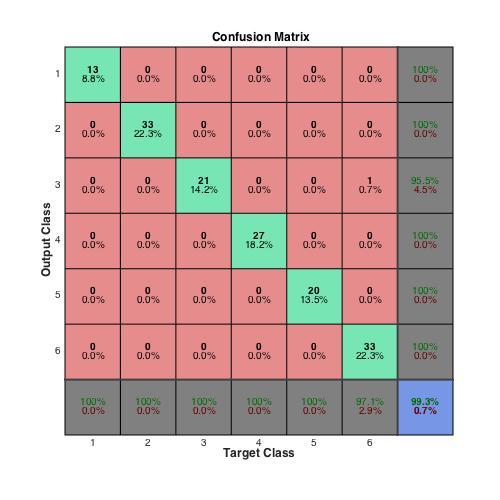
\includegraphics[width=0.5\textwidth]{test_features_ConfusionPlot}
      \caption{Test set confusion plot for the Network trained on the All feature set}
  \label{fig:1}
\end{figure}

\begin{figure}[h!]
  \centering
    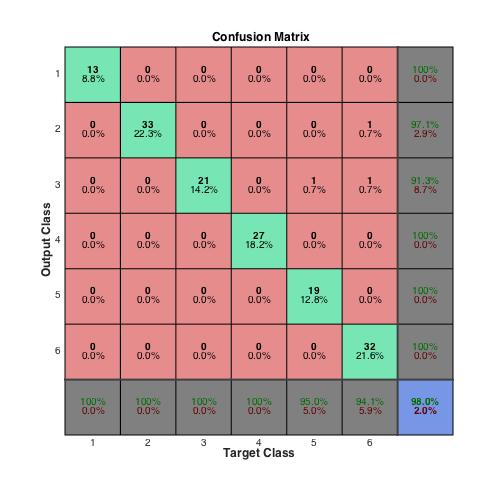
\includegraphics[width=0.5\textwidth]{test_feature_func_confusionPlot}
    \caption{Test set confusion plot Network trained on the Func feature set}
     \label{fig:2}
\end{figure}

Figure \ref{fig:1} and figure \ref{fig:2} show the confusion plots for the test data set for the highest scoring All-Net and Func-Net, respectively. As a result of the high deviation of the highest scoring Func-Net (98\% test data accuracy) from the mean (91.62\% test data accuracy), as opposed to the rather low deviation in case of the All-Net, one might conclude that in case of the Func feature set, the error function being minimised is more susceptible to local minima.

\begin{figure}[h!]
  \centering
    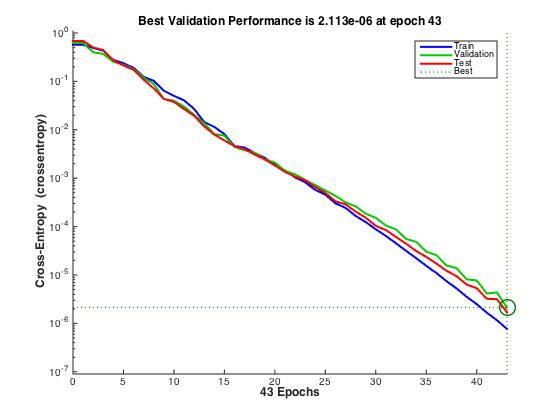
\includegraphics[width=0.5\textwidth]{Full_Feat_PerformancePlot}
      \caption{Plot performance for the network trained on the All feature set}
  \label{fig:3}
\end{figure}

\begin{figure}[h!]
  \centering
    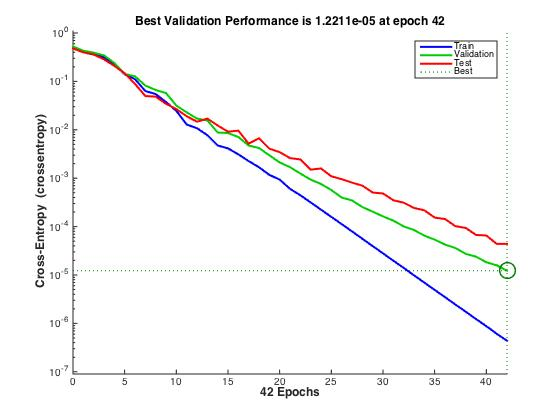
\includegraphics[width=0.5\textwidth]{feature_func_PerformancePlot}
    \caption{Plot performance for the network trained on the Func feature set}
     \label{fig:4}
\end{figure}

Figure \ref{fig:3} and figure \ref{fig:4} show the decrease in training, test and validation error as plotted against the number of epochs for the highest scoring All-Net and Func-Net respectively. While the two plots seem to be similar, figure \ref{fig:4} reveals a much lower entropy error as well as a much higher generalisation capability for the All-Net compared to the Func-Net.

\section{Conclusion}

In this work on authorship attribution, I compared the performance of back propagation fully-connected feedforward neural networks trained on different feature sets. One feature set was comprised of common word frequencies, namely, the count of the 50 most frequent function words in each of the training samples (Func feature set). The other feature set consisted of a combination of token-level features, syntactic features, features based on vocabulary richness and common word frequencies: average word-length, readability, part-of-speech tags frequency distribution as well as the aforementioned 50 most frequent function words, adding up to a total of 90 features (All feature set).

Given this data set, it was found that the neural network structure yielding the highest results was: 50 and 90 input nodes for the Func and All set of features, respectively, 10 nodes in the hidden layer, and 6 output nodes � a node for each author.

 It was found that the neural network trained on the All data set was superior to the neural network trained on the Func data set in terms of both, generalisation capability as well as classification accuracy (an average of 98.33\% vs. 84.67\% on the training samples, and an average of  98.81\% vs. 91.62\% on the test samples).

\bibliography{example_paper}
\bibliographystyle{icml2010}

\end{document} 


% This document was modified from the file originally made available by
% Pat Langley and Andrea Danyluk for ICML-2K. This 2010 version was
% created by Thorsten Joachims & Johannes Fuernkranz, 
% slightly modified from the 2009 version by Kiri Wagstaff and 
% Sam Roweis's 2008 version, which is slightly modified from 
% Prasad Tadepalli's 2007 version which is a lightly 
% changed version of the previous year's version by Andrew Moore, 
% which was in turn edited from those of Kristian Kersting and 
% Codrina Lauth. Alex Smola contributed to the algorithmic style files.  


